\documentclass[letterpaper]{article} % DO NOT CHANGE THIS
\usepackage{aaai24}  % DO NOT CHANGE THIS
\usepackage{times}  % DO NOT CHANGE THIS
\usepackage{helvet}  % DO NOT CHANGE THIS
\usepackage{courier}  % DO NOT CHANGE THIS
\usepackage[hyphens]{url}  % DO NOT CHANGE THIS
\usepackage{graphicx} % DO NOT CHANGE THIS
\urlstyle{rm} % DO NOT CHANGE THIS
\def\UrlFont{\rm}  % DO NOT CHANGE THIS
\usepackage{natbib}  % DO NOT CHANGE THIS AND DO NOT ADD ANY OPTIONS TO IT
\usepackage{caption} % DO NOT CHANGE THIS AND DO NOT ADD ANY OPTIONS TO IT
\usepackage{subcaption}
\frenchspacing  % DO NOT CHANGE THIS
\setlength{\pdfpagewidth}{8.5in}  % DO NOT CHANGE THIS
\setlength{\pdfpageheight}{11in}  % DO NOT CHANGE THIS
\usepackage{array}
%
% These are recommended to typeset algorithms but not required. See the subsubsection on algorithms. Remove them if you don't have algorithms in your paper.
\usepackage{algorithm}
\usepackage{algorithmic}

%
% These are are recommended to typeset listings but not required. See the subsubsection on listing. Remove this block if you don't have listings in your paper.
\usepackage{newfloat}
\usepackage{listings}
\DeclareCaptionStyle{ruled}{labelfont=normalfont,labelsep=colon,strut=off} % DO NOT CHANGE THIS
\lstset{%
	basicstyle={\footnotesize\ttfamily},% footnotesize acceptable for monospace
	numbers=left,numberstyle=\footnotesize,xleftmargin=2em,% show line numbers, remove this entire line if you don't want the numbers.
	aboveskip=0pt,belowskip=0pt,%
	showstringspaces=false,tabsize=2,breaklines=true}
\floatstyle{ruled}
\newfloat{listing}{tb}{lst}{}
\floatname{listing}{Listing}
%
% Keep the \pdfinfo as shown here. There's no need
% for you to add the /Title and /Author tags.
\pdfinfo{
/TemplateVersion (2024.1)
}

% DISALLOWED PACKAGES
% \usepackage{authblk} -- This package is specifically forbidden
% \usepackage{balance} -- This package is specifically forbidden
% \usepackage{color (if used in text)
% \usepackage{CJK} -- This package is specifically forbidden
% \usepackage{float} -- This package is specifically forbidden
% \usepackage{flushend} -- This package is specifically forbidden
% \usepackage{fontenc} -- This package is specifically forbidden
% \usepackage{fullpage} -- This package is specifically forbidden
% \usepackage{geometry} -- This package is specifically forbidden
% \usepackage{grffile} -- This package is specifically forbidden
% \usepackage{hyperref} -- This package is specifically forbidden
% \usepackage{navigator} -- This package is specifically forbidden
% (or any other package that embeds links such as navigator or hyperref)
% \indentfirst} -- This package is specifically forbidden
% \layout} -- This package is specifically forbidden
% \multicol} -- This package is specifically forbidden
% \nameref} -- This package is specifically forbidden
% \usepackage{savetrees} -- This package is specifically forbidden
% \usepackage{setspace} -- This package is specifically forbidden
% \usepackage{stfloats} -- This package is specifically forbidden
% \usepackage{tabu} -- This package is specifically forbidden
% \usepackage{titlesec} -- This package is specifically forbidden
% \usepackage{tocbibind} -- This package is specifically forbidden
% \usepackage{ulem} -- This package is specifically forbidden
% \usepackage{wrapfig} -- This package is specifically forbidden
% DISALLOWED COMMANDS
% \nocopyright -- Your paper will not be published if you use this command
% \addtolength -- This command may not be used
% \balance -- This command may not be used
% \baselinestretch -- Your paper will not be published if you use this command
% \clearpage -- No page breaks of any kind may be used for the final version of your paper
% \columnsep -- This command may not be used
% \newpage -- No page breaks of any kind may be used for the final version of your paper
% \pagebreak -- No page breaks of any kind may be used for the final version of your paper
% \pagestyle -- This command may not be used
% \tiny -- This is not an acceptable font size.
% \vspace{- -- No negative value may be used in proximity of a caption, figure, table, section, subsection, subsubsection, or reference
% \vskip{- -- No negative value may be used to alter spacing above or below a caption, figure, table, section, subsection, subsubsection, or reference

\usepackage{enumitem}
\usepackage{nameref}
\usepackage{adjustbox}
\graphicspath{{./img/}}
\usepackage{multirow}
\usepackage{amsmath}


\setcounter{secnumdepth}{0} %May be changed to 1 or 2 if section numbers are desired.

% The file aaai24.sty is the style file for AAAI Press
% proceedings, working notes, and technical reports.
%

% Title

% Your title must be in mixed case, not sentence case.
% That means all verbs (including short verbs like be, is, using,and go),
% nouns, adverbs, adjectives should be capitalized, including both words in hyphenated terms, while
% articles, conjunctions, and prepositions are lower case unless they
% directly follow a colon or long dash
\title{Pre-processing proposals for plankton images classification}
\author{
    %Authors
    % All authors must be in the same font size and format.
    % Written by AAAI Press Staff\textsuperscript{\rm 1}\thanks{With help from the AAAI Publications Committee.}\\
    % AAAI Style Contributions by Pater Patel Schneider,
    % Sunil Issar,\\
    Lorenzo Serafini\textsuperscript{\rm 1},\\
    Michele Sprocatti\textsuperscript{\rm 2}, %\equalcontrib,
    Alberto Pasqualetto\textsuperscript{\rm 3} %\equalcontrib,
}
\affiliations{
    %Affiliations
    % \textsuperscript{\rm 1}Association for the Advancement of Artificial Intelligence\\
    % If you have multiple authors and multiple affiliations
    % use superscripts in text and roman font to identify them.
    % For example,

    Department of Information Engineering, University of Padua\\
    Via Gradenigo 6, 35131 Padova, Italy\\
    % email address must be in roman text type, not monospace or sans serif
    % proceedings-questions@aaai.org
    \{lorenzo.serafini.1\textsuperscript{\rm 1}, michele.sprocatti\textsuperscript{\rm 2}, alberto.pasqualetto.2\textsuperscript{\rm 3}\}@studenti.unipd.it
%
% See more examples next
}

%Example, Single Author, ->> remove \iffalse,\fi and place them surrounding AAAI title to use it
\iffalse
\title{My Publication Title --- Single Author}
\author {
    Author Name
}
\affiliations{
    Affiliation\\
    Affiliation Line 2\\
    name@example.com
}
\fi

\iffalse
%Example, Multiple Authors, ->> remove \iffalse,\fi and place them surrounding AAAI title to use it
\title{My Publication Title --- Multiple Authors}
\author {
    % Authors
    First Author Name\textsuperscript{\rm 1,\rm 2},
    Second Author Name\textsuperscript{\rm 2},
    Third Author Name\textsuperscript{\rm 1}
}
\affiliations {
    % Affiliations
    \textsuperscript{\rm 1}Affiliation 1\\
    \textsuperscript{\rm 2}Affiliation 2\\
    firstAuthor@affiliation1.com, secondAuthor@affilation2.com, thirdAuthor@affiliation1.com
}
\fi


\begin{document}
\nocopyright

\maketitle

\begin{abstract}
This paper introduces a new image pre-processing technique specifically designed for classifying plankton images with AlexNet.
It enforces the use of the unsharp method and the application of padding before resizing the images in input to the network. It compares the results with other pre-processing methods found in the literature.
\end{abstract}


\section{Introduction} \label{sec:introduction}
Due to their tiny size, plankton often appears in low-quality and low-resolution images. This makes automatic classification challenging.
Thus pre-processing techniques can be employed to overcome these limitations by highlighting the most important features of the plankton, such as shape and texture. In the end, it will result in a better-performing input for the neural network.


\section{Dataset} \label{sec:dataset}
\textit{ZooScan} \cite{digitalZooplanktonGorsky2010} comprises 3771 images captured in the Bay of Villefranche-sur-mer using Zooscan technology. These images are classified into 20 categories, with varying sample sizes ranging from 28 to 427 images per category. The majority of categories encompass zooplankton, various Medusae species, and zooplankton eggs, while the remaining categories consist of non-zooplankton organisms and images with poor focus.

The dataset is split into two folds: for each fold the net is trained with 80\% of the patterns and the remaining 20\% is used to evaluate the model.

The images have different dimensions but all of them consist of pixels with an 8-bit depth and three color channels.
The background of all images is consistently defined by the white color, expressed as RGB(255, 255, 255).


\section{Network} \label{sec:network}
We fed the images into an AlexNet (scheme in figure \ref{fig:AlexNet}) where we replaced the last 3 layers with a fully connected layer using a SoftMax activation function.
The network requires input images with dimension $227 \times 227 \times 3$. It was trained on the provided dataset for 30 epochs.


\section{Method} \label{sec:method}
When we apply the resize operation, since some images have a dimension significantly larger than others, we squeeze the image and lose the plankton morphology: this can lead to a misrepresentation of the pattern.
A comparison of an image resized with and without padding is shown in figure \ref{fig:comparisonPaddingOrNot}.
\begin{figure}[h]
    \centering
    \begin{subfigure}{0.45\textwidth}
        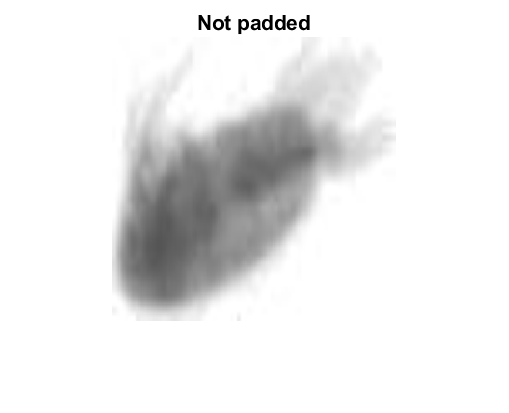
\includegraphics[width=\textwidth]{EX2_only_resized_41_84.png}
        \caption{An image from the dataset resized to $227 \times 227$}
    \end{subfigure}
    \begin{subfigure}{0.45\textwidth}
        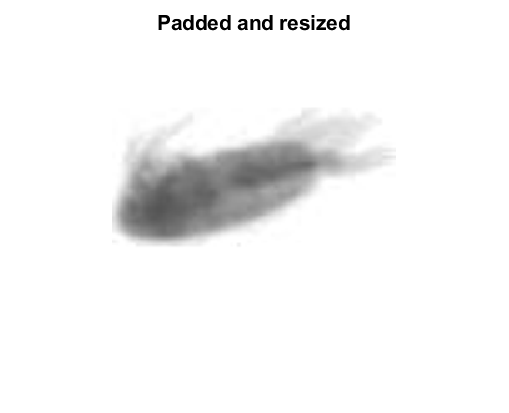
\includegraphics[width=\textwidth]{EX2_padded_and_resized_41_84.png}
        \caption{Same image from the dataset padded before resizing to $227 \times 227$}
    \end{subfigure}
    \caption{Comparison of an image resize with and without padding}
    \label{fig:comparisonPaddingOrNot}
\end{figure}
To avoid incurring this problem, we added white padding to the smaller dimension of the image obtaining a square image of $\max(height, width) \times \max(height, width)$ size.
In this way, the resizing to $227 \times 227$ would not cause the squeezing effect.

Our idea for the preprocessing of the plankton images is to increase the contrast of the image in order to better visualize the details and enhance the transitions in it.
Applying histogram equalization to the whole image was not effective since a major part of the image consists of the white background: for this reason the gray and darker pixels were set to black or very close to it after the equalization, obtaining the opposite effect instead of enhancing the differences in pixel values.
A comparison of an image with and without histogram equalization is shown in figure \ref{fig:comparisonHistogramEqualization}.
\begin{figure}[h]
    \centering
    \begin{subfigure}{0.45\textwidth}
        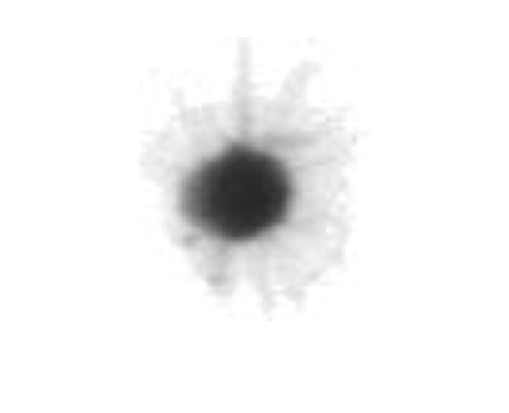
\includegraphics[width=\textwidth]{histeq_gray_orig_ex_07.png}
        \caption{An image from the dataset}
    \end{subfigure}
    \begin{subfigure}{0.45\textwidth}
        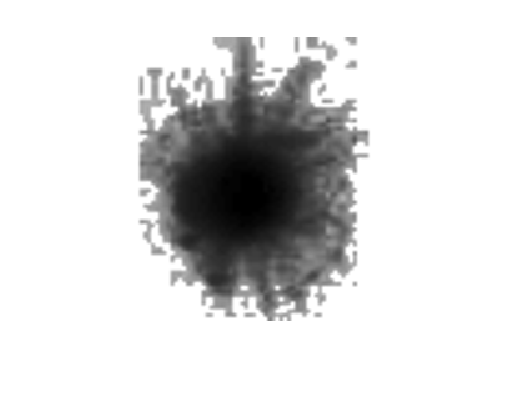
\includegraphics[width=\textwidth]{histeq_ex_07.png}
        \caption{Same image from the dataset with histogram equalization applied: contrast is lost}
    \end{subfigure}
    \caption{Comparison of an image with and without histogram equalization}
    \label{fig:comparisonHistogramEqualization}
\end{figure}
Knowing this behavior we tried to apply local methods like Local Histogram Equalization and local laplacian filtering, but both of them did not improve the accuracy of the network, on the contrary, the results were worse than the ones obtained without any pre-processing (accuracy of about $0.82$): for LHE we achieved an accuracy of about $0.78$, for local laplacian filtering an accuracy of about $0.79$.

The Unsharp method is the one that worked best, the name comes from the fact that it produces a blurred version of the image and uses it to increase the contrast between neighboring pixels and highlight the transitions.
This method blurs the image with a Gaussian filter, calculates the difference image between the original and the blurred one, and ultimately sums the original image with the difference image multiplied by a constant called "amount" following the formula:
\begin{equation*}
    sharpened = original + (original - blurred) \times Amount.
\end{equation*}

The Matlab \texttt{imsharpen} function's parameters $Radius$ (the standard deviation of the Gaussian blur) and $Amount$ have been set after a validation process where the training set is composed by 60\% of the images and the validation set by 20\% of the images, the remaining is used afterward to evaluate the model.
After the validation process, the dataset was split 80/20 as explained in section \nameref{sec:dataset} by merging the training and validation splits, finally, the net was trained with the best parameters found.


\section{Results} \label{sec:results}
As can be seen in table \ref{tab:accuracy}, \citeauthor{hybridPreprocessingDai2017}'s pre-processing method is not effective using AlexNet architecture.

The Unsharp method, while not providing a significant improvement in accuracy, is the best pre-processing method among the ones tested.

On the other hand, applying padding before resizing the images has a positive effect on the accuracy of the net, increasing it by about 2\%.

\begin{table}[H]
    \centering
    \begin{tabular}{|c c|c c|}
        \hline
        \multicolumn{2}{|c|}{\multirow{2}{*}{Method}} & \multicolumn{2}{c|}{Accuracy} \\
                                                & & No Padding & Padding \\
        \hline
        \multirow{2}{*}{No pre-processing}   & Fold 1    & 0.81457 & 0.85298 \\
                                            & Fold 2    & 0.83311 & 0.83179 \\
        \hline
        \multirow{2}{*}{\citealt{hybridPreprocessingDai2017}}      & Fold 1    & 0.80397 & 0.85298 \\
                                            & Fold 2    & 0.81325 & 0.78808 \\
        \hline
        \multirow{2}{*}{Unsharp mask}      & Fold 1    & 0.81854 & 0.86490 \\
                                            & Fold 2    & 0.83179 & 0.83576 \\
        \hline
    \end{tabular}
    \caption{Accuracy of the net with various pre-processing methods}
    \label{tab:accuracy}
\end{table}

The resulting confusion matrices are shown in figure \ref{fig:comparisonConfusionMatrix}.


\section{Conclusions} \label{sec:conclusions}
In this paper, we presented a new image pre-processing approach for classifying plankton images with AlexNet.
The results show that Unsharp is the best pre-processing method that we tested for increasing the accuracy of the network even though not providing a very significant gain in performance.
The usage of padding, instead, is the key to gaining some percentage points in accuracy.

The combined application of padding and unsharp method allows the network to reach an average accuracy of 85\% on both folds of the given dataset.

\bibliography{refs}

\newpage
\onecolumn

\begin{figure}
    \centering
    \begin{subfigure}{0.45\textwidth}
        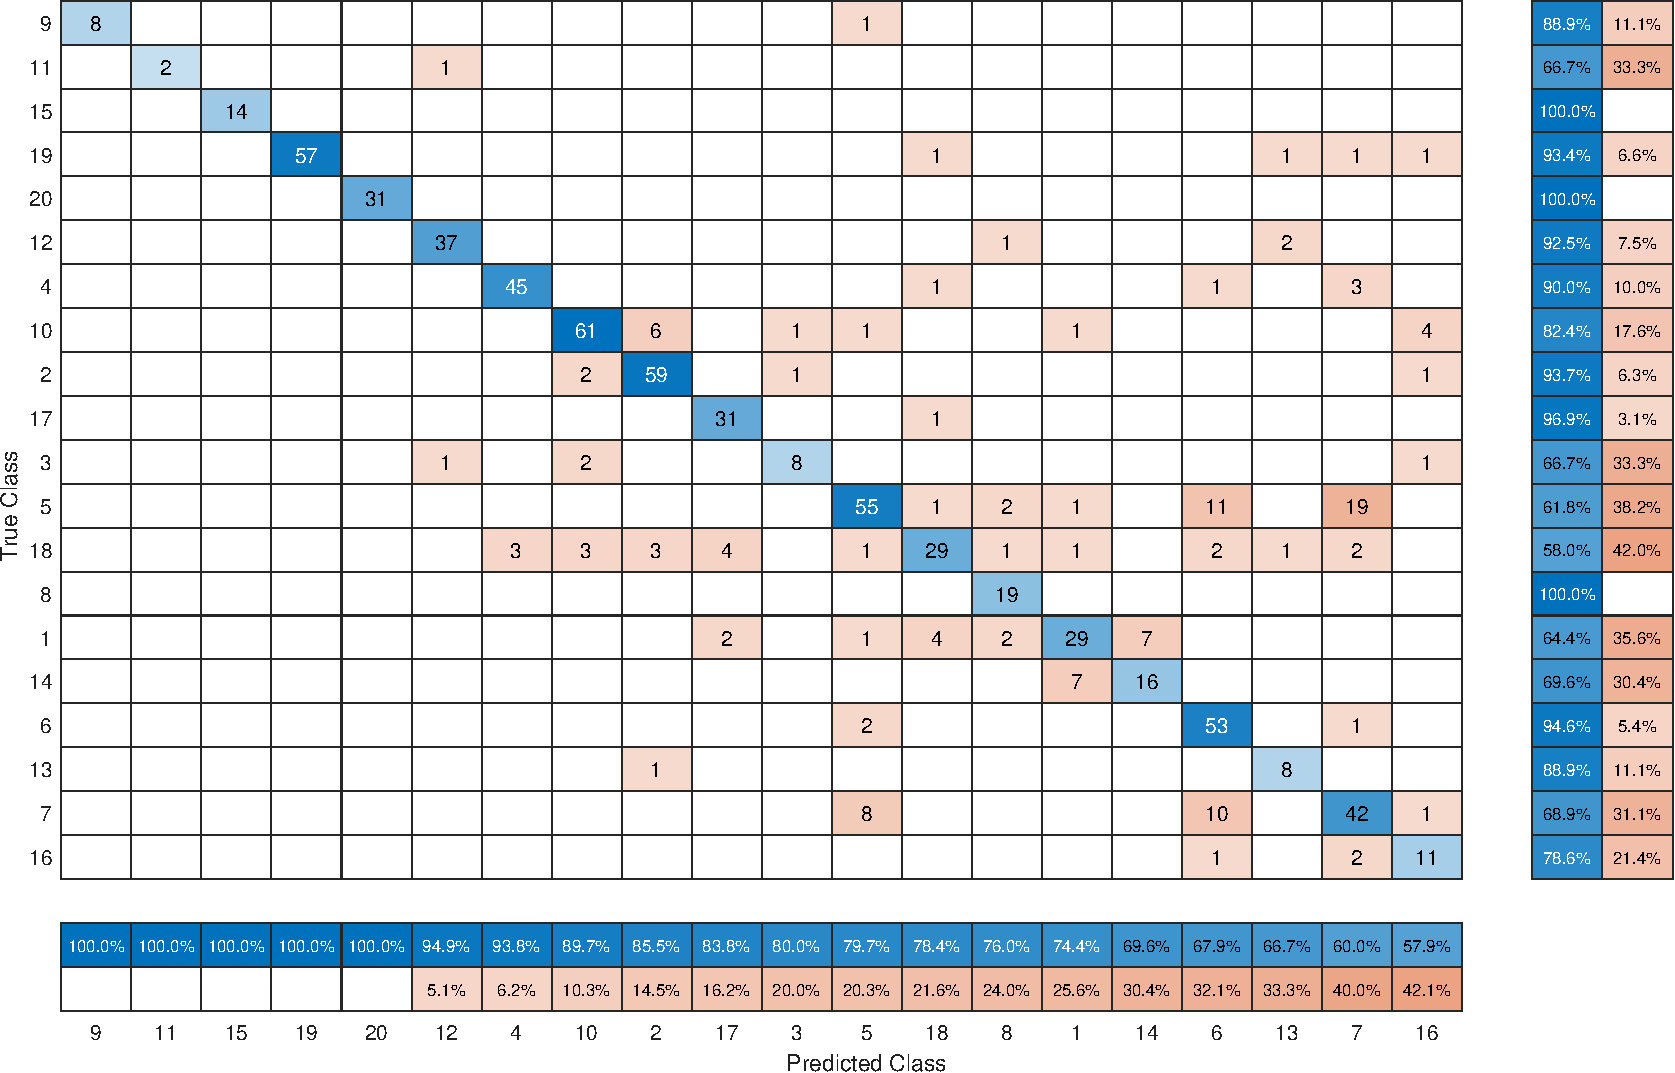
\includegraphics[width=\textwidth,height=0.25\textheight]{No_Preprocessing_fold1_80_20_acc_0.81457.pdf}
        \caption{Confusion Matrix fold 1 without pre-processing}
    \end{subfigure}
    \begin{subfigure}{0.45\textwidth}
        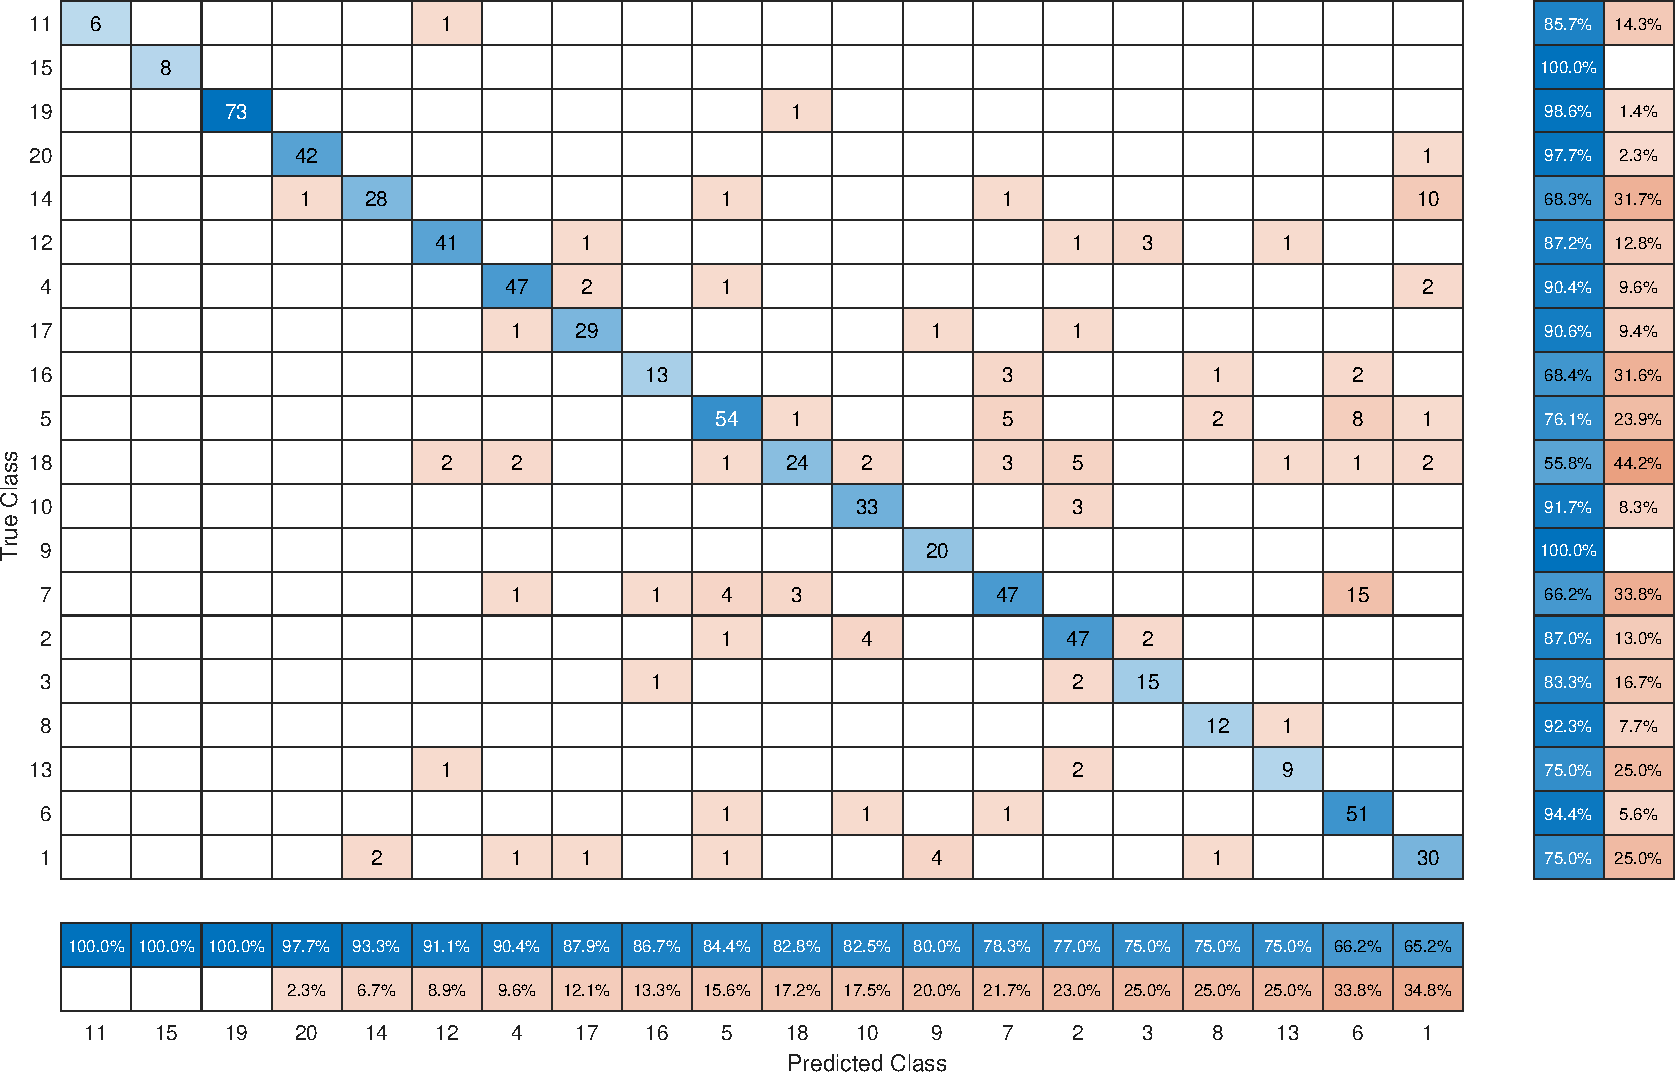
\includegraphics[width=\textwidth,height=0.25\textheight]{No_Preprocessing_fold2_80_20_acc_0.83311.pdf}
        \caption{Confusion Matrix fold 2 without pre-processing}
    \end{subfigure}

    \begin{subfigure}{0.45\textwidth}
        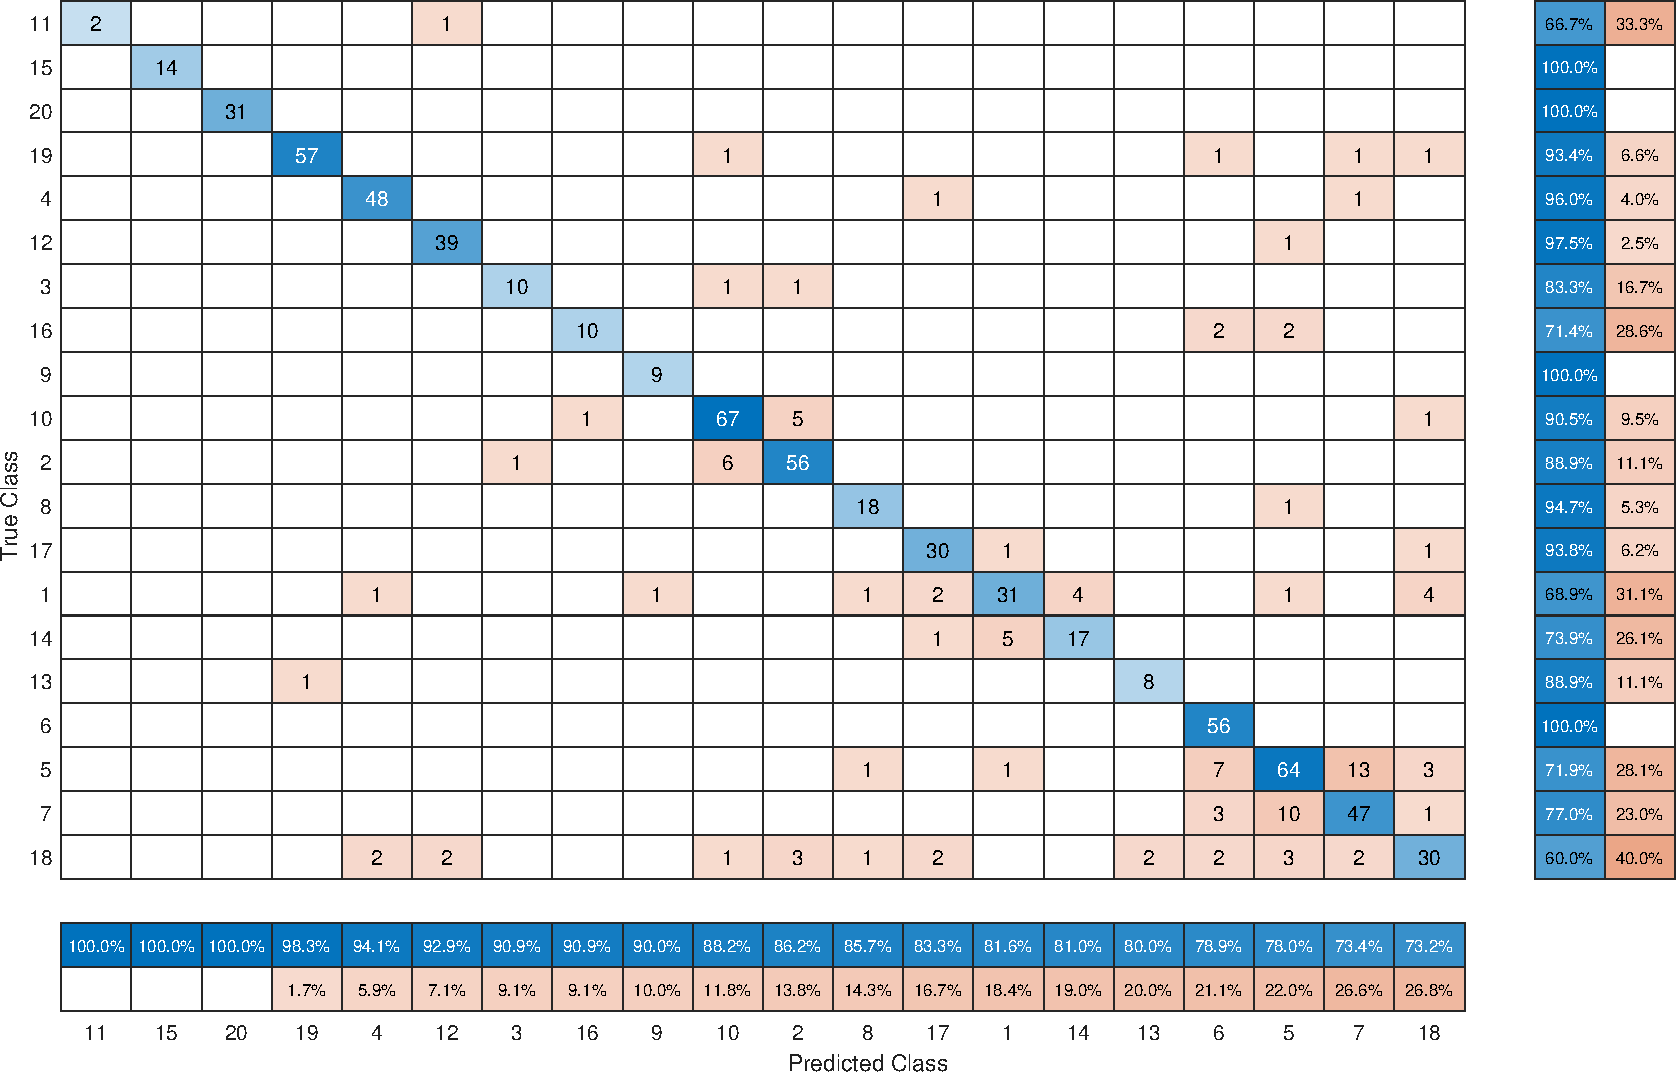
\includegraphics[width=\textwidth,height=0.25\textheight]{No_Preprocessing_fold1_80_20_square_acc_0.85298.pdf}
        \caption{Confusion Matrix fold 1 with square padding}
    \end{subfigure}
    \begin{subfigure}{0.45\textwidth}
        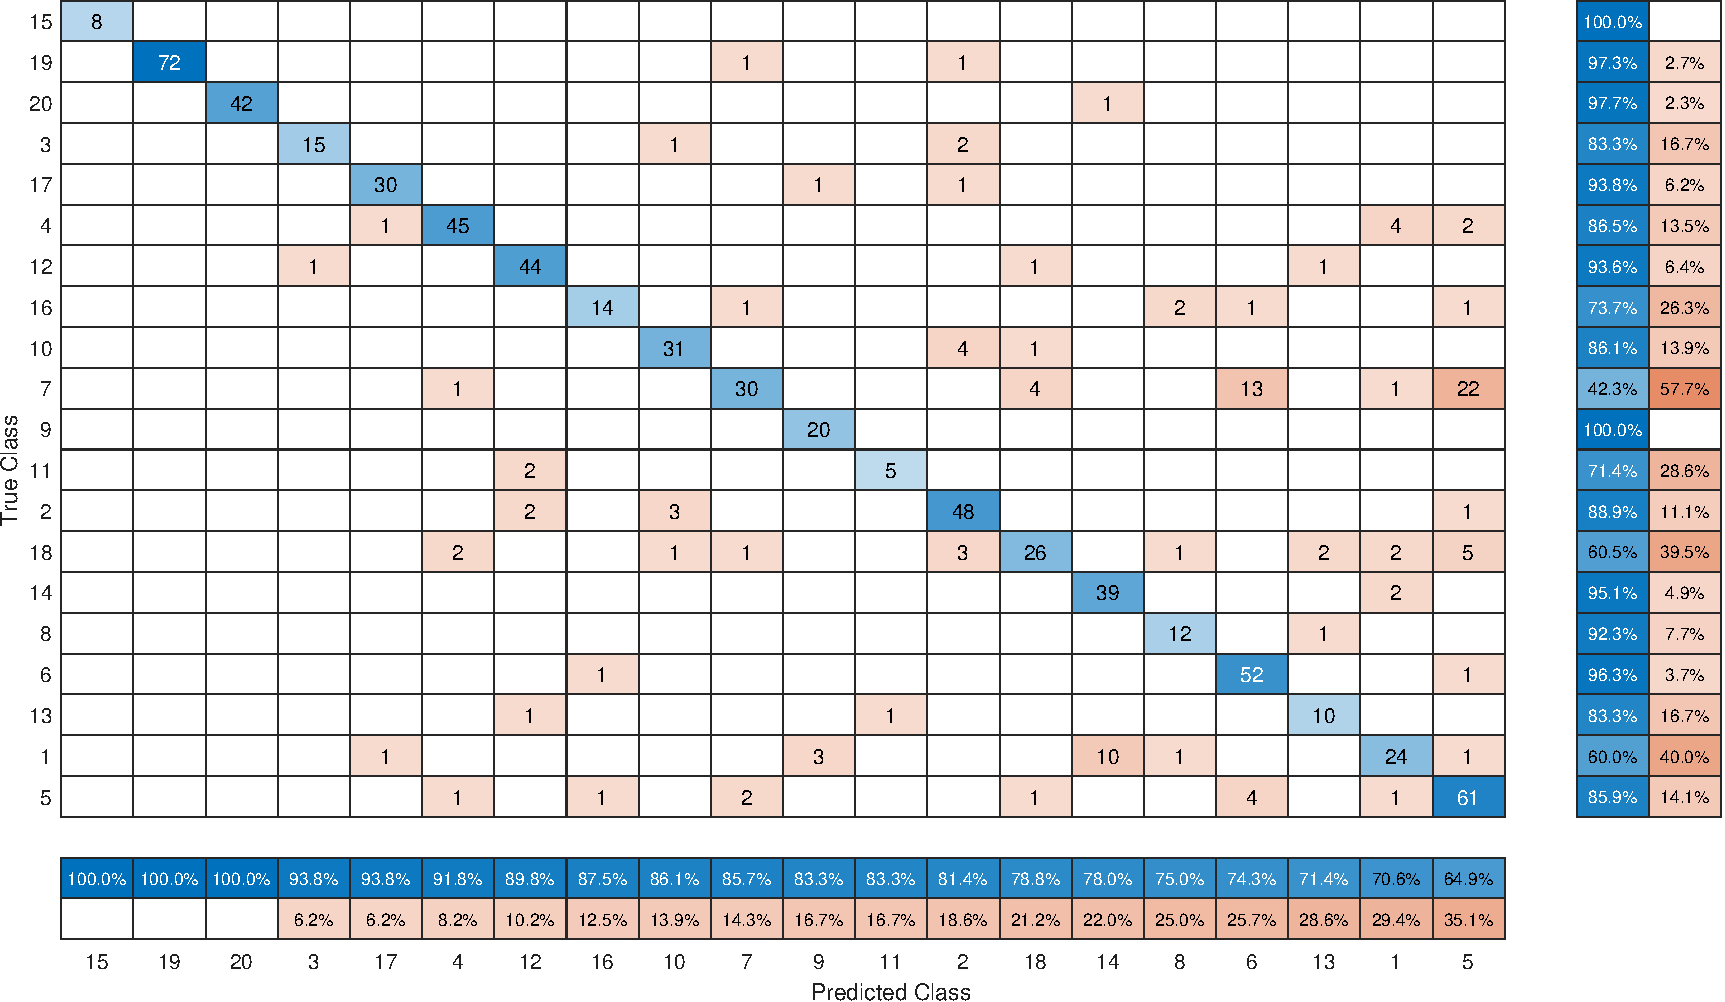
\includegraphics[width=\textwidth,height=0.25\textheight]{No_Preprocessing_fold2_80_20_square_acc_0.83179.pdf}
        \caption{Confusion Matrix fold 2 with square padding}
    \end{subfigure}

    \begin{subfigure}{0.45\textwidth}
        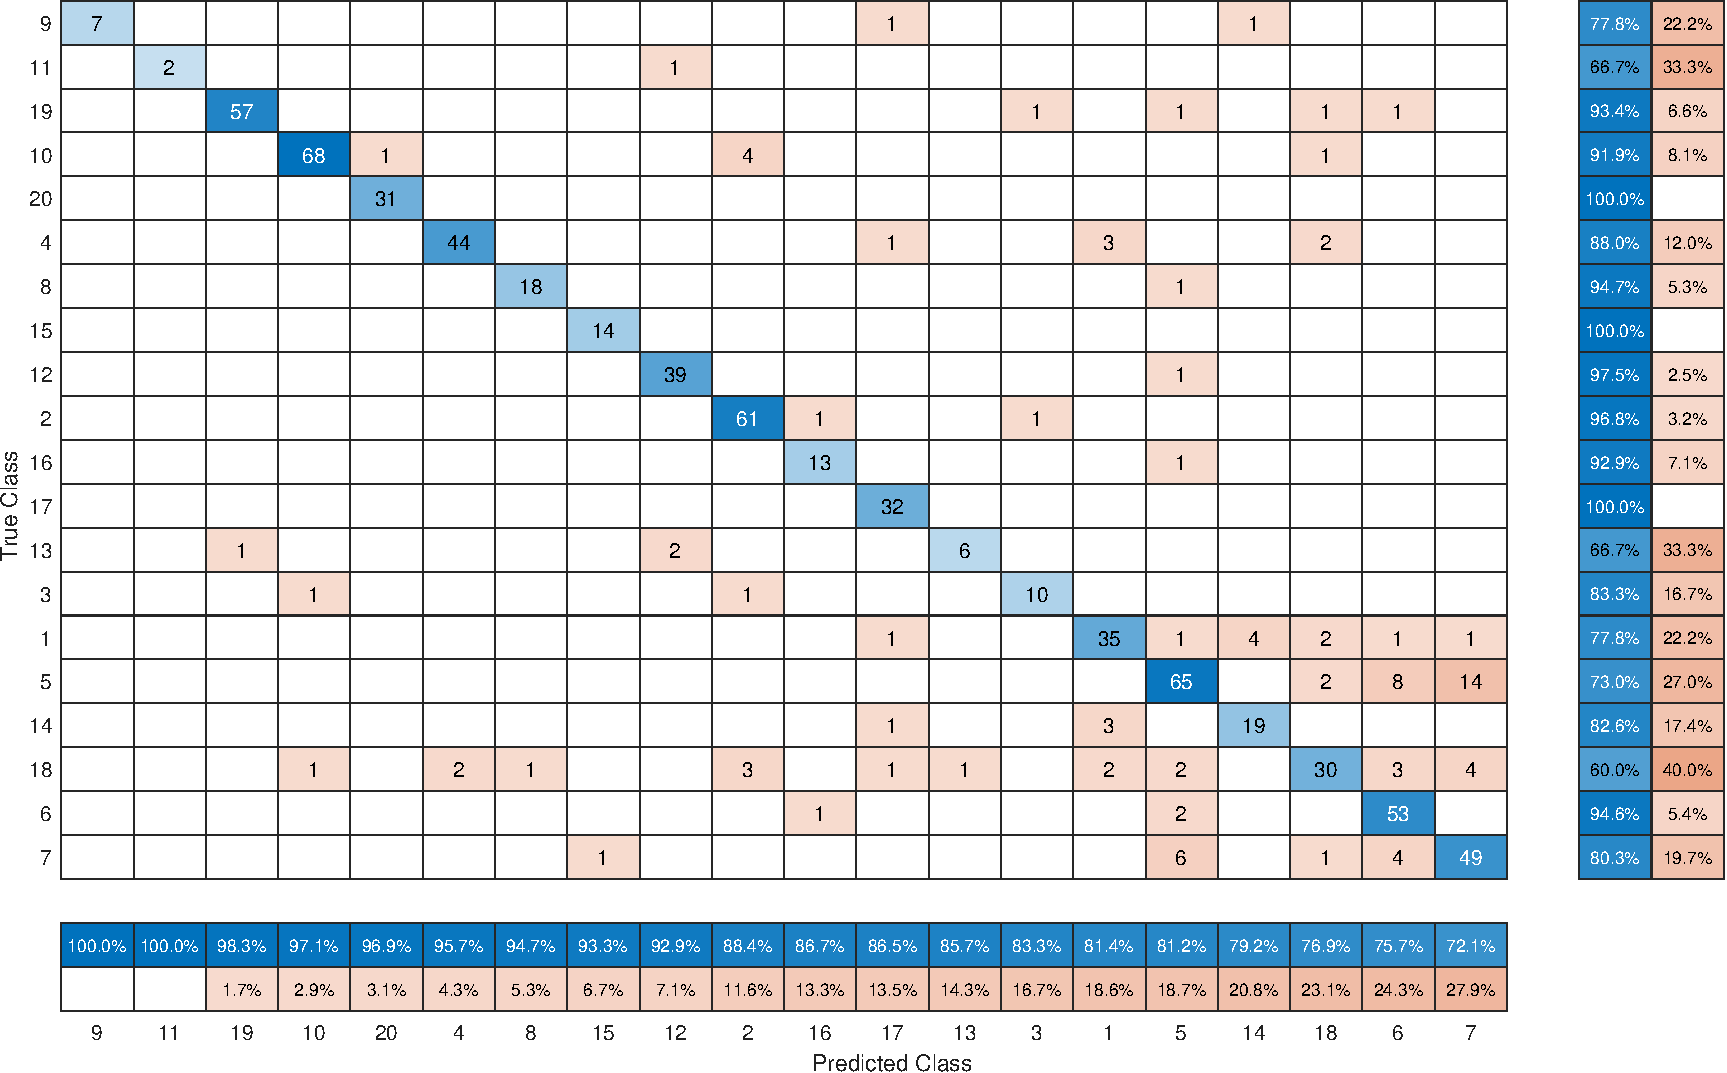
\includegraphics[width=\textwidth,height=0.25\textheight]{FINAL_USH_n_PAD_fold1_acc_0.86490.pdf}
        \caption{Confusion Matrix fold 1 with Unsharp mask and padding pre-processing}
    \end{subfigure}
    \begin{subfigure}{0.45\textwidth}
        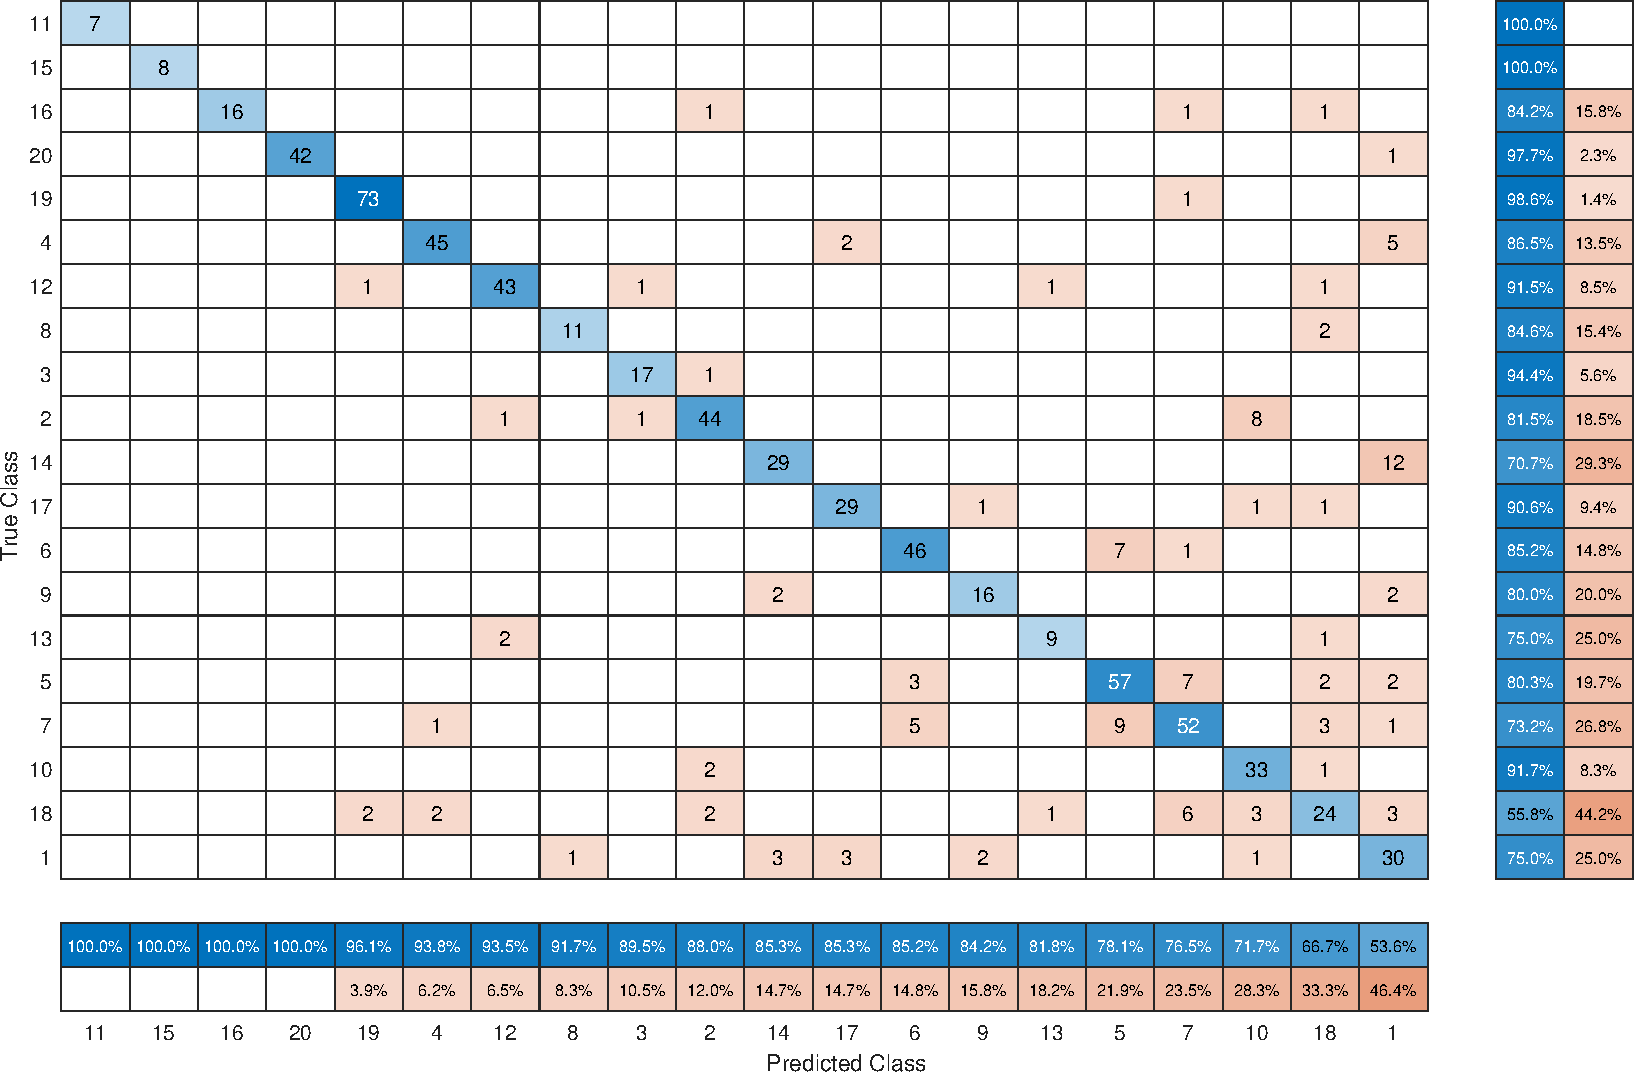
\includegraphics[width=\textwidth,height=0.25\textheight]{FINAL_USH_n_PAD_fold2_acc_0.83576.pdf}
        \caption{Confusion Matrix fold 2 with Unsharp mask and padding pre-processing}
    \end{subfigure}
    \caption{Confusion matrices}
    \label{fig:comparisonConfusionMatrix}
\end{figure}

\newpage

\begin{figure}
    \centering
    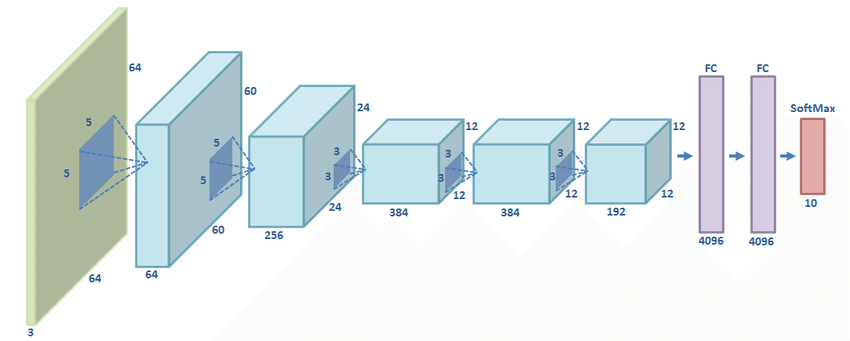
\includegraphics[width=\textwidth]{AlexNet_scheme.png}
    \caption{AlexNet}
    \label{fig:AlexNet}
\end{figure}


\end{document}
